\chapter{Music-related body motion}\label{chap:motion}

`What do you mean by \emph{gesture}?' This is still my standard question whenever I hear the word used in a musical context. The term gesture is frequently used but seldomly defined. The same is the case for several other key terms used to describe the role of the body in musicking. This becomes particularly tricky when working between disciplines. Researchers from, for exmaple, musicology, sociology, performance studies, gesture studies, human-computer interaction, and human movement science use many of the same terms but often with a different meaning. When I first started reading up on the literature in the various fields, I became increasingly confused. Every publication seemed to use different terminology to describe the same phenomena. For example, does a `piano gesture' describe physical motion, the experience of an action, a sonic phrase, or something else? And, when talking about `movement,' does this relate to what can be measured with a motion capture system? In the following, I will define and describe some core terminology.


\section{Motion}

I prefer the term \emph{music-related body motion} when generally describing human bodily activity in a musical context. Such motion is not necessarily \emph{musical}. For example, the motion of a pianist scratching her head while playing is not musical, but it would still be categorized as music-related. I include \emph{body} in the term to avoid ambiguity with other types of music-related motion, such as moving sounds in a spatial audio setup. Finally, \emph{motion} is used in a traditional physics-based sense: the act of moving. In English, two words describe this phenomenon: \emph{motion} and \emph{movement}. They are often used interchangeably, although they have slightly different meanings. The Oxford Dictionary suggests this differentiation:

\begin{description}
\item[Motion:] the action or process of moving or being moved
\item[Movement:] an act of moving
\end{description}

In my mother tongue, Norwegian, we only have one word to describe the act of moving (\emph{bevegelse}). The same is the case in many other Germanic languages. The English words come from Latin, where there are also two different words (\emph{motus} and \emph{motio}). Confusingly, these two words are usually defined as being the same \citep{jacob_acousmatic_2019}. In Italian, on the other hand, there are two distinct meanings of the words \emph{moto} and \emph{movimento}.

Since I do not have an innate feeling for the difference between motion and movement, I often ask native English speakers to explain how they perceive the difference between them. One explanation I got was to look at an old-school clock. The hands of the clock display movement, and this movement is the result of motion. Then one could reason that movement is more related to how the phenomenon is experienced.

\citet{jacob_acousmatic_2019} suggests that different \emph{perspective views} leave flexibility to the way terms are used. This makes it possible to differentiate between linguistically similar yet perceptually different phrases, such as the `movement of the heart' and the `motion of the heart.' The former would be a non-specific and metaphorical description, while the latter relates to the physical displacement of a particular heart. One could say that the `motion of a pianist's hand' can be measured with a motion capture system, while the `movement of a pianist's hand' refers to the experience of how the hand is moving through the air.

Motion thus appears to be the most scientific term and is also the preferred term in physics and its sub-field mechanics. Much physics terminology is used in \emph{biomechanics}, the field that studies the motion of living organisms. However, in human movement science, there seems to be a mix of the terms motion and movement. This may be because human movement science is a field on the intersection between biomechanics, psychology, medicine, and neuroscience. Then there is also a need to describe the body using both physical and psychological terms.

Within biomechanics, two core areas of study are \emph{kinematics} and \emph{dynamics}. The kinematics describes how fast and in which direction an object is moving. We know from school physics that motion can be defined as the continuous displacement of an object in space over time. This assumes that one knows an object's \emph{position} in space, usually represented in a three-dimensional Cartesian space. It is possible to quantify motion by measuring the total \emph{distance traveled} or \emph{displacement} of an object. These are not necessarily identical. For example, if a person walks in a circle, the distance traveled will increase over time. However, the total displacement will be zero each time the person passes the starting point.

How fast an object move is usually measured as its \emph{velocity}, which is a vector quantity equivalent to an object's \emph{speed} and direction. One can say that the speed is related to the distance traveled while the velocity is associated with the displacement. An object's \emph{acceleration} is calculated as the derivative of its velocity. It tells about how much the velocity changes over time. The acceleration helps identify when an object starts and stops and is a measure that is frequently used in (musical) human--computer interaction. It is also possible to look at the \emph{jerk} (the third derivative of position) and the \emph{snap} (the fourth derivative of position). These may seem like abstract concepts, but studies have shown that we can experience both jerk and snap when the acceleration changes \citep{eager_beyond_2016}.


\section{Motion capture}\label{sec:motion-capture}

There are many ways to measure motion, but these can be broken down into two main types of systems: camera-based and sensor-based \citep{jensenius_methods_2018}. Some systems measure an object's position in space, while others measure velocity or acceleration. It is easy to find an object's velocity or acceleration by calculating the first or second derivative of position. It is more challenging to go the other way, that is, calculate position from acceleration.

Since camera-based systems are better at measuring an object's position in space, these are often considered state-of-the-art among motion capture systems. The most reliable systems use multiple infrared cameras positioned around the capture space (Figure~\ref{fig:christina}). The cameras emit infrared light, which is reflected on markers placed on the body of the person or object to be captured. The reflected light is then captured by the cameras and sent to a computer that calculates the exact position through a \emph{triangulation} process. The result is three-dimensional tracking of each of the markers in space. The benefit of such systems is that they can capture at high speeds (more than 100~Hz) and high spatial resolution (in the range of millimeters). The captured points can be visualized directly or used as the basis for further analysis.

\begin{figure}[tbp]
	\centerline{
	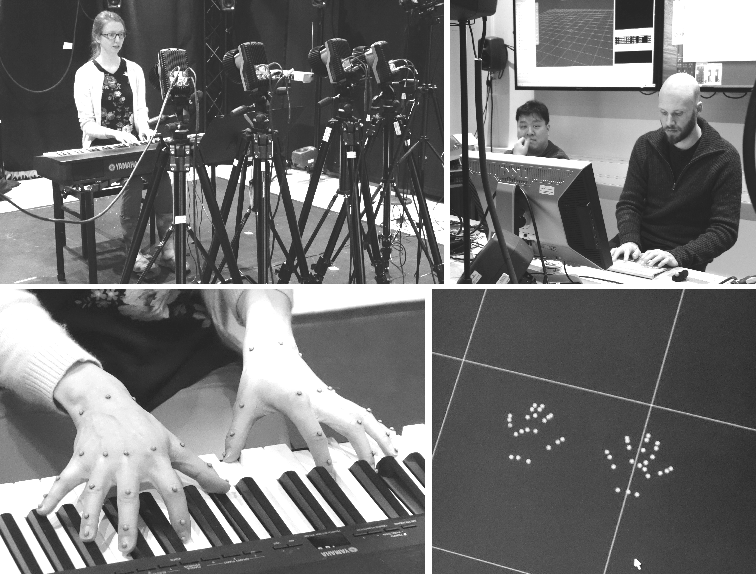
\includegraphics[width=1\textwidth]{figures/19-mocap-crop.pdf}}
	\caption{Setup for optical infrared motion capture of pianist Christina Kobb in the fourMs Lab at University of Oslo. There are multiple cameras placed in front to allow for capturing the small markers placed on the hands (bottom left). The markers can be visualized in a three-dimensional grid in software (bottom right).}
	\label{fig:christina}
\end{figure}

While infrared, marker-based systems are considered state-of-the-art, there are also other camera-based motion tracking solutions. New \emph{computer vision} techniques makes it possible to extract features from regular video recordings \citep{moeslund_survey_2001,moeslund_survey_2006,rautaray_vision_2015}. Also, new camera types help push the field forwards. This includes stereo-cameras that mimic the function of the human eyes and depth-cameras that can measure the distance to objects. New artificial intelligence-based models also allow for capturing full-body motion with a moving camera \citep{voulodimos_deep_2018}.

There are several drawbacks of using camera-based motion capture systems. The price tag is one, although such systems have become more affordable in recent years. More problematic are the constraints enforced by the need to have a camera focused on a particular recording space and that the cameras need to `see' what is going on. This often leads to \emph{occlusion}, meaning that certain areas or markers are invisible to the cameras. For example, a dancer moving close to the floor or a cellist whose instrument covers a large part of the performer's body. Then it is impossible to capture the motion of the whole body accurately.

Many of the problems with camera-based motion capture systems are non-existent in sensor-based systems. There are numerous such systems, based on various types of sensors: acoustic, mechanical, magnetic, inertial, and electrical \citep{bishop_tracking_2001}. Of these, the inertial ones are the most popular for measuring motion. These days, \emph{inertial measurement units} (IMUs) are almost ubiquitous. These sensor units contain \emph{accelerometers} that measure the gravitational pull. This signal can measure the rate of change of motion, although it is not identical to measuring acceleration as the second derivative of the position. This also makes it difficult to calculate the position from accelerometer data without considerable drift \citep{skogstad_comparing_2011}.
IMUs typically also contains \emph{gyroscopes} and a \emph{magnetometer}. A gyroscope measures the rotation of the sensor, and the magnetometer acts as a compass. Together, these three IMU sensors---accelerometer, gyroscope, and magnetometer---allow for capturing both three-dimensional motion and rotation in a small sensor unit.

One compelling feature of inertial sensors is that they are not affected by external factors such as ferromagnetic objects or light. They are also small, cheap, use little power, and can be sampled at high frequencies. Even though they are ubiquitous in consumer electronics, they are not embedded in many commercial musical instruments (yet). However, as reviewed by \citet{medeiros_comprehensive_2014}, many researchers explore their potential in musical applications.


\section{Force}

In the previous section, we only considered the \emph{dynamics} of moving objects. However, for objects to begin (or keep) moving, there needs to be some \emph{force} acting upon them. Newton's second law tells us that the force ($F$) is related to the product of a body's mass ($m$) and acceleration ($a$): $F=ma$. This means that a massive object requires more energy usage to move than a lighter one. Newton's third law tells that two objects exert equal force on each other for objects at rest. This is relevant from an interaction perspective since the \emph{pressure} ($p$) that you use to push on something is related to the amount of force ($F$) used and the area ($A$) that it is used on: $p=F/A$.

The force applied to an object can be measured with a \emph{force-sensing resistor} (FSR). Such sensors are becoming increasingly popular in new musical interfaces since they allow for continuous control of sound features. We will look more at some examples of such usage in later chapters. Force can also be estimated from measuring muscle activity, which has become popular in experimental music devices \citep{tanaka_musical_1993,perez_biotools_2008}. Muscle activity can be detected with \emph{electromyograms} (EMG), and it is particularly effective to use EMG sensors on a musician's arms to pick up information about hand and finger motion \citep{nymoen_mumyo_2015,erdem_exploring_2020}. Figure \ref{fig:myo-usertest} shows an example of an armband with eight integrated EMG sensors used in a musical application. We will look more at other examples of muscle-based performance in Chapter~\ref{sec:muscles}.

Another term from school physics is \emph{friction}, which in its purest form can be defined as $f=\mu N$, where $f$ is the friction force, $\mu$ is the friction coefficient, and $N$ the normal force. Friction is particularly interesting from a musical perspective since it is often the starting point for sound production. For example, the sound of a bowed string stems from the friction between objects and the energy put into the object's motion \citep{guettler_bowed_2002,serafin_sound_2004,schoonderwaldt_mechanics_2009}.

Motion and force are also both related to \emph{haptics}, meaning the sense of touching or being touched. Haptic experiences may be said to consist of both the sense of material properties (tactics) and the motion properties (kinesthetics) of the objects \citep{cook_music_1999}. While haptic experiences are a natural part of acoustic instruments, few electro-acoustic instruments allow for such a sensing modality. Fortunately, several researchers explore haptics in new instrument designs \citep{papetti_musical_2018}.

Perceivers do not generally get a haptic experience, but there have been some experiments with creating haptic-based installations. One example is a series of multimedia installations by \citet{stenslie_virtual_2011}, in which he explored haptic bodysuits. \citet{turchet_smart_2019} tested giving vibrotactile gilets to perceivers in a music performance context. They found that some were positive to such an extended musical experience, while others were not. Clearly, more research and experimentation are needed to figure out if and how haptics can be used to give perceivers a richer musical experience.


\section{Degrees of freedom}\label{sec:dof}

In engineering, one often talks about \emph{degrees of freedom} (DoF) as the number of independent movement variables in a mechanical system. In a typical three-dimensional scenario, a moving object has six degrees of freedom: three translational (X, Y, Z) and three rotational (yaw, pitch, roll) \citep{huston_principles_2008}. However, not all degrees of freedom may be available in all contexts. For example, a hinge has one degree of freedom since it can only rotate around one axis. A slider has two degrees of freedom, and a ball-and-socket machine joint has three.

In instrument acoustics, the concept of degrees of freedom has been used to describe the instrument's sound-producing elements and how they are connected. \citet{chaigne_acoustics_2016} argue that a guitar string can be modeled with two degrees of freedom. This means that the string has one degree of freedom, and the resonator (the guitar's body) also has one. This simplifies a complex interaction but helps explain the core parts of the instrument's interaction.

In a biomechanical system, like the human body, the joints usually work together. To understand the system's motion potential, it is necessary to add up the degrees of freedom from the involved joints. The human body has 17 large parts, and these give us a total of 54 degrees of freedom when moving around \citep{huston_principles_2008}. With all the smaller joints of the body, there are approximately 230 joints in total. Since there are so many variables to consider, it is difficult to calculate the total number of degrees of freedom of the body. In any case, it may be more interesting to look at the degrees of freedom of the interaction in question.

The degrees of freedom of a (bio)mechanical system is related---but not similar---to the system's number of \emph{control dimensions}. By control dimensions, I mean the degrees of freedom of a physical instrument that corresponds to the degrees of freedom of the performer's body parts. For example, a one-dimensional finger joint cannot exploit the three-dimensional possibilities of a ball-and-socket-based joystick. Therefore, the control dimensions of an instrument will be lower than the separate degrees of freedom of the instrument and the performer. Take the case of the cello, an instrument that allows for a high level of `expressivity.' The cello is an instrument that is considered difficult to master. However, \citet{rowe_machine_2001} argues that a cellist only has four degrees of freedom in performance: bow force, bow velocity, bow distance from the bridge, and finger position on the fingerboard. I would argue that string selection could be a fifth control dimension, but we are still talking about a low number of control dimensions. So the complexity of mastering to play the cello is not due to its degrees of freedom. Similarly, developing instruments with higher structural complexity does not automatically lead to `better' interaction.

Calculating the control dimensions of an instrument is not a straightforward procedure. For example, one could argue that an individual piano key only has one degree of freedom: key-down and key-up. The keys are touch-sensitive, so the velocity with which one hits the key directly influences the sound level. There are many keys to choose from, but selecting an individual key could be considered one more control dimension. The pianist, therefore, has two control dimensions: which key to play and the velocity and force used in the attack. These dimensions are called \emph{pitch} and \emph{velocity} in the MIDI protocol (we will get back to a discussion of MIDI in Chapter~\ref{sect:midi}). In addition to the keys, the piano also has two or three pedals that can alter the sound level and timbral qualities.

The organ has a similar keyboard interface to the piano, but its control dimensions differ. An organ player also makes a key selection but does not have velocity control on the keys. The sound level is controlled separately from the keys by adjusting the airflow to the organ pipes. On the other hand, in the organ, it is possible to change the timbre of the sound by adding or removing pipes. So even though the piano and organ share the same pitch control interface (the keyboard), they differ in the other control dimensions (sound level and timbre).

As we shall see in Chapter~\ref{sec:seaboard}, new keyboard-based interfaces allow for multidimensional control on each key. This radically changes how a keyboard-based instrument can be played. An interesting question then arises: is the total number of control dimensions that much different in practice? The limited number of control dimensions on each piano key is compensated by playing many keys simultaneously. It is no problem to play chord progressions with 5--8 keys on the piano. My experience is that I tend to focus on only playing on 1--3 keys simultaneously on multidimensional keyboards. I do not have the cognitive capacity to control more than a few multidimensional keys continuously.


\section{Action}\label{sec:action}

The control dimensions of an instrument is an example of how we can apply a techno-cognitive approach to the analysis of an interaction between a human and an instrument. This is based on investigating what can be measured objectively (the number of instrument or body parts) and how these can be used in performance. \emph{Action} is another techno-cognitive term. It is related to motion, but it is not the same. Motion describes the physical displacement of an object in time and space. This displacement can be measured objectively with a motion capture system. In my thinking, motion is a continuous phenomenon. Everything is always in motion, from the atomic to the galaxic level. In nature, motion does not have a beginning and end; it just \emph{is}. Therefore, it does not make sense to talk about `a motion.' As soon as we segment the continuous motion signal into a temporal segment, we interpret it as a time-limited action. Action is a subjective entity.

Let us carry out a small thought experiment to clarify the difference between motion and action. Imagine a drummer performing an individual stroke on a snare drum. You will easily be able to identify this as a single action: the performer lifts the stick, hits the snare drum, and returns to rest. If performed in a continuous flow, it would be perceived as one coherent action. If you were to measure this action with a motion capture system, however, you would get a continuous signal describing the position of the drummer's hand. When does the action begin and end? This is a matter of interpretation. The motion capture recording will display a physical motion representation from the beginning to the end of the capture session. There is nothing in the motion capture data that will inform about the action. You may look at the graph and locate where you believe that the action began and ended. However, this is your subjective interpretation of the observed motion. The motion capture data can reveal the exact height of the stick, but it will not tell when the action started and stopped.

I think about an action as a \emph{spatiotemporal} phenomenon. Space and time are merged in my mental representation of the action in question. To have a way of representing this on paper, I started experimenting with video visualization techniques \citep{jensenius_video_2013}. One example of a video visualization can be seen in the \emph{motion history images} of a series of individual drum strokes in Figure~\ref{fig:figures_samkopf}. I made this visualization from a continuous video recording of individual drum strokes. The segmentation into separate images is based on a threshold applied to the \emph{quantity of motion} calculated from the video sequence. The assumption was that an action would start after the percussionist had stood still for a second or two between strokes. The segmented video clips were `averaged' into one motion history image. Each of these images then represents one action, at least according to my interpretation of the sequence. Time is indirectly represented through the spatial and temporal distribution of the motion. It is impossible to see precisely \emph{when} something happened, as when plotting motion capture data along a time axis. But you get a compact visual representation of the action as a coherent spatiotemporal unit.

\begin{figure}[tbp]
	\centering
		\includegraphics[width=\columnwidth]{figures/20-percussion.jpg}
	\caption{Motion history images created from a video recording of a percussionist performing individual drum strokes on a pad. Each image represents around 15 seconds of video material and can be seen as a way of representing the spatiotemporal characteristics of the individual actions.}
	\label{fig:figures_samkopf}
\end{figure}

As the above example showed, an action may be understood as a holistic unit---or a \emph{chunk}---of motion or force \citep{buxton_chunking_1986}. Such an action chunk is subjective, meaning that people may perceive actions differently. In cognition in general, and music cognition in particular, we may talk about three temporal levels, each related to the three main memory functions: \emph{sensory}, \emph{short-term}, and \emph{long-term} memory \citep{snyder_music_2000}. Based on such a tri-part division, \citet{godoy_reflections_2008} has suggested three levels of chunking:

\begin{itemize}
	\item[Sub-chunk level:] the perception of continuous sound and motion features. This is based on sensory memory and covers events up to 0.5 seconds.
	\item[Chunk level:] the perception of fragments of sound and motion that are perceived holistically, such as sound objects and goal-directed actions. This is based on short-term memory and is typically between 0.5 to 5 seconds.
	\item[Supra-chunk level:] the perception of several chunks concatenated into larger structures. This is based on long-term memory and covers events longer than 5 seconds.
\end{itemize}

Humans handle these levels effortlessly and in parallel. For example, we may observe the instantaneous unfolding of sound and motion while at the same time keeping an internal memory of the trajectories of a sequence and an overall image of extended patterns. Analyzing the same with a computer-based system reveals the complexity of this multi-layered parsing task.
Particularly challenging is that action chunks are context-dependent, meaning we perceive them relative to what happened before or after. They can also be `nested;' several actions that follow each other may be perceived as one large action. For example, playing a scale run on a piano can be considered a series of separate actions if we focus on each finger's motion. If we instead look at the motion of the hand or the upper body, a scale run can be perceived as one coherent action chunk. Then we may talk about the effect of \emph{coarticulation} \citep{hardcastle_coarticulation_1999}, the merging of individual units into larger supra-units (Figure~\ref{fig:coarticulation}).

\begin{figure}[tbp]
	\centerline{
	\includegraphics[width=.7\textwidth]{figures/21-coarticulation-crop.pdf}}
	\caption{Sketch of motion over time of individual goal-directed actions (A), and how they will overlap if performed so close together that they prefixes and suffixes overlap (B). This would result in the coarticulation of the action trajectories (C) (based on \citep{aramaki_understanding_2014}).}
	\label{fig:coarticulation}
\end{figure}

From an interaction perspective, we may think of actions as `foreground' activities in a continuous motion stream. Then it also makes sense to talk about a `background,' motion outside our attention. This is sometimes called \emph{fidgeting} and can be defined as actions that are peripheral or nonessential to the main task \citep{mehrabian_analysis_1986}. We may even think of fidgeting as `motion noise,' which is typically filtered out when one deals with action recognition. That said, looking into noise can reveal relevant features. I have for some years been interested in human \emph{micromotion}, the tiniest motion that humans can produce and perceive. This I have done through motion capture studies of people standing still while listening to silence and music \citep{jensenius_exploring_2017,gonzalez_sanchez_correspondences_2018,gonzalez_sanchez_analysis_2019,zelechowska_headphones_2020}. In these studies, the participants were explicitly told not to do anything, just to stand still. The aim was to look at the motion of their standstill and see if we could find systematic behavioral patterns. We are here talking about motion at a scale up to around 10 mm/s. We have found that there are, indeed, systematic differences in people's motion patterns. The nature of motion and its relationship to musical features is still under active research. My scientific investigation into human micromotion is tightly connected to artistic explorations into sonic microinteraction, which we will look at in Chapter~\ref{sec:sverm}.

Figure~\ref{fig:fidgeting} is an attempt to summarize how I think about the differences between the objective terms motion and force and the subjective concepts action and fidgeting. Note that an action can be based on either motion or force. It is possible to see muscle tension without measuring any motion. For example, try pressing your fingers against a table. You can feel the exertion of force, but there will be no motion. This is an example of a motionless action. Similarly, there may be motion without any exerted force. However, the most important is distinguishing between what is measurable (motion and force) and what can only be inferred from the measurements (action and fidgeting).

\begin{figure}[tp]
\includegraphics[width=1\columnwidth]{figures/22-fidgeting-crop.pdf}
\caption{A sketch of the relationships between motion/force, action, and fidgeting. Motion is the continuous displacement in time and space. Actions are subjective motion chunks, while fidgeting refers to the `motion noise' between actions. Actions may coarticulate into larger action units.}
\label{fig:fidgeting}
\end{figure}


\section{Gesture}

The last term to define at this stage---and also the most complex one---is  \emph{gesture}. %The way I will use the term in this book is as the meaning of an action.
This is a term that has received growing interest in recent decades among music researchers \citep{gritten_music_2006,gritten_new_2011}. Around 20 years ago, \citet{cadoz_gesture-music_2000} wrote a summary of different types of gesture definitions in music and music interaction. I contributed with an updated review ten years later \citep{jensenius_musical_2010} and a study of how the term gesture was used in the music technology community \citep{jensenius_gesture_2014}.
The main finding from these review studies was that the gesture is used broadly. Some use it more or less synonymous with what I call motion, others with action, and others again in a more linguistic sense.

I prefer to think about gesture the way it is used in linguistics and behavioral studies, what \citet[p.7]{kendon_gesture_2004} refers to as `visible action as utterance.' In my thinking, a gesture is related to conveying \emph{meaning} through action. Meaning should here be understood broadly, and can---as we will get back to later---also be expressive. The main point is that a gesture is not only physical motion or any goal-directed action; it is part of human communication. \citet[p.12-19]{mcneill_hand_1992} proposed a taxonomy of different gestural functions:

\begin{itemize}
\item \emph{Iconics} represent a particular feature of an object and can be described in terms of the gesture's shape and spatial extent. Iconic gestures are often used to illustrate an action, such as imitating a knocking movement with a hand while saying `knocking on the door.'
\item \emph{Metaphorics} are similar to iconics but represent an abstract feature of an object. An example of a metaphoric gesture may be saying `something happened' while holding up the hands to refer to `something.'
\item \emph{Beats} occur together with spoken words to highlight discontinuities and to stress specific words. Beats are typically carried out as in/out or up/down actions and may be seen as emphasizing the most important words in a narrative.
\item \emph{Deictics} indicates a point in space, for example, pointing in a specific direction while saying `over there.'
\item \emph{Emblems} are stereotypical patterns with an agreed meaning, such as waving `good-bye' or the `thumbs up' sign.
\end{itemize}

McNeill's gesture theory is built on the idea that gestures coexist with speech. This is not to say that they have to co-occur, but instead that gestures and speech are \emph{co-expressive}. Here, \citet[p.15]{mcneill_gesture_2005} argues that `language is inseparable from imagery' and that mental imagery is embodied in the gestures that co-occur with speech.
To explain the relationships between gesture and speech, \citet[p.37]{mcneill_hand_1992} outlines what he calls the \emph{Kendon continuum}, based on the typology of gestures suggested by \citet{kendon_gesticulation_1980}: \emph{gesticulation}, \emph{emblems}, \emph{pantomime} and \emph{sign language}. As shown in Figure~\ref{fig:continuum}, this continuum covers two extremes: \emph{gesticulation} denotes gestures that always co-occur with speech and \emph{sign language} the linguistically self-contained ones.

\begin{figure}[tp]
\includegraphics[width=\columnwidth]{figures/23-kendon-crop.pdf}
\caption{A sketch of the \emph{Kendon continuum} shows how different types of gestures relate to speech \citep[7]{mcneill_gesture_2005}.}
\label{fig:continuum}
\end{figure}


\section{Musical gesture}

The literature on relationships between gesture and speech is relevant when moving into the realm of music. In the music literature, gesture is used in many different ways. For example, \citet{bielawski_instrumentalmusik_1979} proposed a model in which he refers to an instrument as a `transformer' of gestures. While there are also others that use the gesture more or less synonymous with motion or action, most think about higher abstraction levels. \citet[p.16]{metois_musical_1997} proposes this definition:

\begin{quote}
[B]oth [physical and auditory gestures] present the ability to communicate musical intentions at a higher level than an audio wave form. The similarity of their level of abstraction motivated the author to label them both as Musical Gestures.
\end{quote}

\citet[p.95]{hatten_interpreting_2004} argues that a musical gesture is `significant energetic shaping through time.' He primarily refers to the experience of musical gesture `within' music, either through the score or the musical sound. Then I find it easier to relate to the definition proposed by \citet[p.xx]{gritten_music_2006}:

\begin{quote}
[A] gesture is a movement or change in state that becomes marked as significant by an agent. This is to say that for movement or sound to be(come) gesture, it must be taken intentionally by an interpreter, who may or may not be involved in the actual sound production of a performance, in such a manner as to donate it with the trappings of human significance.
\end{quote}

This definition suggests a flow of communication between the performer and the perceiver. The performer's motion `becomes' a gesture if the perceiver understands it. An interesting question then arises regarding consciousness: does an action have to be carried out consciously to be seen as a gesture? From a communication perspective, \citet[p.15]{kendon_gesture_2004} argues that gestures are intentional and therefore have to be carried out consciously. On the other hand, \citet[162]{gritten_music_2006} suggest that a musical gesture can be perceived significant even if performed unconsciously.
This is related to how \citet{murray-rust_towards_2011} talk about \emph{musical acts}. In their model, a musical act needs to be (a) embodied, (b) have an intention, and (c) be intelligible. If one person acts and is not understood by another, then it fails to impact.
I would argue that we should open for ambiguity. The same action can be perceived as either intentional or unintentional by different people. In any case, we have to think of a gesture as a subjective entity.

In my thinking, the gesture concept boils down to what in traditional Saussarian semiotics would be seen as a separation between \emph{sign} and \emph{signifier}. We can separate between the \emph{meaning} of a gesture---broadly speaking---and the motion involved in communicating that meaning. For example, think about the gesture of waving `good-bye' to someone. This gesture can be performed with or without speech, but it would nevertheless contain the meaning of saying `good-bye.' You can wave with the left hand or right hand, or both. The physical motion would be different, but the meaning (hence the gesture), would be the same.

One prominent example of a musical gesture can be seen in cartoon films. Think of when a character falls off a cliff accompanied by a long glissando illustrating the downwards motion of the character, possibly ending with a massive `bang' when the character hits the ground. Here, meaning is attached to the sound, which is also directly related to visible (or imaginary) action. The sound may evoke motion imagery, even if nothing is seen on the screen.

There are also examples of how meaningful motion may lead to sonic imagery. Think of a pianist playing the final notes of a classical piano concerto. The performance ends with a majestic final chord, which the pianist holds while listening to the decaying sound. The pianist may continue to hold the chord long after the sound has become inaudible, say, for three more seconds, before finally lifting the hands high up in the air and back to rest position before taking the applause. Such a motion-based gesture creates suspense and prolongs the experience of the piano sound.

Figure~\ref{fig:gesture} sums up how a musical gesture can be related to the continuous motion and sound on the physical side and the perceptual actions and sound objects on the perceptual side. In some cases, a musical gesture may be driven primarily by sound, like in the cartoon case mentioned above. Other times, a gesture may be primarily connected to motion, like in the piano example. However, in most cases, musical gestures are based on the combination of sound and motion.

\begin{figure}[tbp]
			\includegraphics[width=\columnwidth]{figures/24-musical-gesture-crop.pdf}
			\caption{A visual summary of relationships between the continuous flow of motion and sound, the chunking of motion and sound into actions and sound objects, and how the two may be experienced as a musical gesture.}
			\label{fig:gesture}
\end{figure}


\section{Position, posture, and pose}

The concepts of motion, action, and gesture are all related to moving bodies. It is also useful to describe bodies that are not in motion. Here I suggest to differentiate between \emph{position}, \emph{posture}, and \emph{pose}. Position is the most technical of these, which I will use to describe the physical location of a body, a body part, or an object in space. The position is something that can be measured with a motion capture system. Then we can look at the motion capture data and find that a person's foot was located on the floor 1157~x~432~x~920 millimeters from the center point in the XYZ coordinate system used in the space. Looking at different points in time, it is then possible to find the various positions that a person has been standing in over the recording.

I will use posture as a subjective term to describe how a person holds their body. A person's `base' posture defines how they stand, and can be easily recognized. Posture is also something that one can develop over time through exercise. Think, for example, about how you can learn to make a `power posture.' It may be possible to calculate the spatial features of a posture based on position data, but this would require a subjective placement/selection of the points from which the individual positions were captured. So posture is related to the position in a similar way that action is related to motion.

Finally, I will use the term pose to refer to postures with a meaning-bearing component. They are often intentional and are typically something that is used in performance. As such, one may say that a pose is based on communication without moving. This is similar to a gesture, with the main difference being that gestures are dynamic while poses are static. Poses also typically refer to how the whole body is organized, although one may argue that setting up a pose with only the hands or head is possible. Lifting your nose, for example, can be seen as a pose to behave `snobbish.' There may also be cases during which a pose and a gesture overlap. Many people would probably consider a `thumbs up' sign to be a gesture. I would agree with that if it is dynamic, that is, if you are lifting your hand in a particular way to show the thumb. However, if you only consider the `thumbs up' as a static sign, I would instead call it a pose.

My main point here is that both gestures and poses need to be interpreted to be understood.
So-called gesture or pose recognition systems will need to start by capturing position or motion. Then one needs to segment these continuous data streams into postures and actions before finally trying to infer their meaning-bearing components. In the case of `musical gesture systems,' one also needs to consider the sound. First, the continuous sound needs to be recorded before it can be segmented into `perceivable' sound objects. Finally, these sound objects can be combined with information about actions to understand the meaning of a musical gesture. This is a non-trivial task, and many researchers work on this topic from different angles. We will look more at some of my explorations in a discussion of air instruments in Chapter~\ref{chap:touchless}.
